\documentclass[]{article}
\usepackage{lmodern}
\usepackage{amssymb,amsmath}
\usepackage{ifxetex,ifluatex}
\usepackage{fixltx2e} % provides \textsubscript
\ifnum 0\ifxetex 1\fi\ifluatex 1\fi=0 % if pdftex
  \usepackage[T1]{fontenc}
  \usepackage[utf8]{inputenc}
\else % if luatex or xelatex
  \ifxetex
    \usepackage{mathspec}
  \else
    \usepackage{fontspec}
  \fi
  \defaultfontfeatures{Ligatures=TeX,Scale=MatchLowercase}
\fi
% use upquote if available, for straight quotes in verbatim environments
\IfFileExists{upquote.sty}{\usepackage{upquote}}{}
% use microtype if available
\IfFileExists{microtype.sty}{%
\usepackage{microtype}
\UseMicrotypeSet[protrusion]{basicmath} % disable protrusion for tt fonts
}{}
\usepackage[margin=1in]{geometry}
\usepackage{hyperref}
\hypersetup{unicode=true,
            pdftitle={Chapter 8: The Method of Least Squares},
            pdfborder={0 0 0},
            breaklinks=true}
\urlstyle{same}  % don't use monospace font for urls
\usepackage{graphicx,grffile}
\makeatletter
\def\maxwidth{\ifdim\Gin@nat@width>\linewidth\linewidth\else\Gin@nat@width\fi}
\def\maxheight{\ifdim\Gin@nat@height>\textheight\textheight\else\Gin@nat@height\fi}
\makeatother
% Scale images if necessary, so that they will not overflow the page
% margins by default, and it is still possible to overwrite the defaults
% using explicit options in \includegraphics[width, height, ...]{}
\setkeys{Gin}{width=\maxwidth,height=\maxheight,keepaspectratio}
\IfFileExists{parskip.sty}{%
\usepackage{parskip}
}{% else
\setlength{\parindent}{0pt}
\setlength{\parskip}{6pt plus 2pt minus 1pt}
}
\setlength{\emergencystretch}{3em}  % prevent overfull lines
\providecommand{\tightlist}{%
  \setlength{\itemsep}{0pt}\setlength{\parskip}{0pt}}
\setcounter{secnumdepth}{5}
% Redefines (sub)paragraphs to behave more like sections
\ifx\paragraph\undefined\else
\let\oldparagraph\paragraph
\renewcommand{\paragraph}[1]{\oldparagraph{#1}\mbox{}}
\fi
\ifx\subparagraph\undefined\else
\let\oldsubparagraph\subparagraph
\renewcommand{\subparagraph}[1]{\oldsubparagraph{#1}\mbox{}}
\fi

%%% Use protect on footnotes to avoid problems with footnotes in titles
\let\rmarkdownfootnote\footnote%
\def\footnote{\protect\rmarkdownfootnote}

%%% Change title format to be more compact
\usepackage{titling}

% Create subtitle command for use in maketitle
\newcommand{\subtitle}[1]{
  \posttitle{
    \begin{center}\large#1\end{center}
    }
}

\setlength{\droptitle}{-2em}

  \title{Chapter 8: The Method of Least Squares}
    \pretitle{\vspace{\droptitle}\centering\huge}
  \posttitle{\par}
  \subtitle{Joseph Sepich}
  \author{}
    \preauthor{}\postauthor{}
    \date{}
    \predate{}\postdate{}
  

\begin{document}
\maketitle

{
\setcounter{tocdepth}{2}
\tableofcontents
}
\section{Problem 1 Simplest problem using least squares
method}\label{problem-1-simplest-problem-using-least-squares-method}

\subsection{a. Find the constant function that best fits the
data.}\label{a.-find-the-constant-function-that-best-fits-the-data.}

\[
\begin{array}{c|c|c|c|} 
x & -1 & 2 & 3\\
y & \frac54 & \frac43 & \frac5{12}\\
\end{array}
\]

A constant function is of the form \(f(x) = c\), so in this case we are
looking for a value of c that minimizes the error function:

\[\psi(c) = \Sigma(f(x_k) - y_k)^2 = \Sigma(c - y_k)^2\]

In order to minimize this function, the derivative \(\frac{d\psi}{dc}\)
must be zero. So we get the normal equation:

\[\Sigma2(c - y_k)=0\]

We can rewrite this as:

\[(m+1)c = \Sigma y_k\]

We know we have \(m+1 = 3\) and \(\Sigma y_k = 3\).

\[3*c = 3\] \[c = 1\]

So our constant function of best fit is \(f(x) = 1\).

\subsection{b. Find the value c such that the function f(x) = c best
approximates the
data.}\label{b.-find-the-value-c-such-that-the-function-fx-c-best-approximates-the-data.}

This is again using a constant equation as a line of best fit to our
data. We have the following data and normal equation from the previous
problem.

\[\Sigma2(c - y_k)=0\]

We can rewrite this as:

\[(m+1)c = \Sigma y_k\]

\[
\begin{array}{c|c|c|c|} 
x & 1.4 & 1.5 & 1.4\\
y & -0.1 & 0 & 0.1\\
\end{array}
\]

With \(m+1 = 3\) and \(\Sigma y_k = 0\), we can fill in our normal
equation:

\[3*c = 0\] \[c = 0\]

This makes our line of best fit:

\[f(x) = c = 0\]

\section{Problem 2 MLS with polynomial
regression}\label{problem-2-mls-with-polynomial-regression}

\subsection{a. What straight line best fits the following data (using
least
squares)?}\label{a.-what-straight-line-best-fits-the-following-data-using-least-squares}

\[
\begin{array}{c|c|c|c|c|} 
x & 1 & 2 & 3 & 4\\
y & 0 & 1 & 1 & 2\\
\end{array}
\]

We can use the normal equations that we dervied similarly to the
constant equation in the last example:

\[\Sigma x_k^2*a + \Sigma x_k * b = \Sigma x_k * y_k\]
\[\Sigma x_k * a + (m + 1)*b = \Sigma y_k\]

Let's calculate our values:

\[
\begin{array}{c|c|} 
m+1 & 4\\
\Sigma x_k^2 & 30\\
\Sigma x_k & 10\\
\Sigma x_k*y_k & 13\\
\Sigma y_k & 4
\end{array}
\]

This gives us the following matrix:

\[
\left(\begin{array}{cc} 
30 & 10\\
10 & 4
\end{array}\right)
\left(\begin{array}{c} 
a \\
b 
\end{array}\right) =
\left(\begin{array}{c}
13 \\
4 
\end{array}\right)
\]

Solving this matrix we get:

\[
\left(\begin{array}{cc} 
1 & 0\\
0 & 1
\end{array}\right)
\left(\begin{array}{c} 
a \\
b 
\end{array}\right) =
\left(\begin{array}{c}
0.6 \\
-0.5 
\end{array}\right)
\]

This means our line of best fit is:

\[f(x) = 0.6x - 0.5\]

\subsection{b. Using MLS represent the data as a parabolic
function.}\label{b.-using-mls-represent-the-data-as-a-parabolic-function.}

In this case instead of using \(y = ax + b\) for our line of best fit,
we use \(y = ax^2 + b\). This means we must adapt our normal equation,
since the partial derivative of our error function with respect to a
will change. Our new normal functions will be:

\[\Sigma x_k^4*a + \Sigma x_k^2 * b = \Sigma x_k^2 * y_k\]
\[\Sigma x_k^2 * a + (m + 1)*b = \Sigma y_k\]

Now let's use our data to fill in the values that we need.

\[
\begin{array}{c|c|c|c|} 
x & -1 & 0 & 1\\
y & 3.1 & 0.9 & 2.9\\
\end{array}
\]

\[
\begin{array}{c|c|} 
m+1 & 3\\
\Sigma x_k^2 & 2\\
\Sigma x_k^4 & 2\\
\Sigma x_k^2y_k & 6\\
\Sigma y_k & 6.9
\end{array}
\]

This gives us the following matrix:

\[
\left(\begin{array}{cc} 
2 & 2\\
2 & 3
\end{array}\right)
\left(\begin{array}{c} 
a \\
b 
\end{array}\right) =
\left(\begin{array}{c}
6 \\
6.9 
\end{array}\right)
\]

Solving this matrix we get:

\[
\left(\begin{array}{cc} 
1 & 0\\
0 & 1
\end{array}\right)
\left(\begin{array}{c} 
a \\
b 
\end{array}\right) =
\left(\begin{array}{c}
2.1 \\
0.9 
\end{array}\right)
\]

This means our parabolic line of best fit is: \[y = 2.1x^2 + 0.9\]

\subsection{c. Find the values a and b such that the function g(x) =
ax+b best approximates the
data.}\label{c.-find-the-values-a-and-b-such-that-the-function-gx-axb-best-approximates-the-data.}

\[
\begin{array}{c|c|c|c|} 
x & 1.4 & 1.5 & 1.4\\
y & -0.1 & 0 & 0.1\\
\end{array}
\]

Here we once again are using a linear function as the line of best fit.
We can use our normal functions:

\[\Sigma x_k^2*a + \Sigma x_k * b = \Sigma x_k * y_k\]
\[\Sigma x_k * a + (m + 1)*b = \Sigma y_k\]

Now let's use our data to fill in the values that we need.

\[
\begin{array}{c|c|} 
m+1 & 3\\
\Sigma x_k^2 & 6.17\\
\Sigma x_k & 4.3\\
\Sigma x_ky_k & 0\\
\Sigma y_k & 0
\end{array}
\]

This gives us the following matrix:

\[
\left(\begin{array}{cc} 
6.17 & 0\\
0 & 3
\end{array}\right)
\left(\begin{array}{c} 
a \\
b 
\end{array}\right) =
\left(\begin{array}{c}
0 \\
0 
\end{array}\right)
\]

Solving this matrix we get:

\[
\left(\begin{array}{cc} 
1 & 0\\
0 & 1
\end{array}\right)
\left(\begin{array}{c} 
a \\
b 
\end{array}\right) =
\left(\begin{array}{c}
0 \\
0 
\end{array}\right)
\]

Meaning that we still get the constant equation that we got for the same
data in the first problem in this homework set of \(y=0 = 0*x + 0\).

\section{Problem 3 MLS Non-Polynomial
Functions}\label{problem-3-mls-non-polynomial-functions}

\subsection{a.}\label{a.}

We are given a data set (\(x_k, y_k\)) with k = 0,\ldots{},m. We seek a
function of the form:

\[g(x) = \alpha sin(x) + \beta cos(x)\]

that best approximates the data. Set up the normal equations, which
solve the problem with the method of least squares.

In order to derive normal functions we must first write out our error
function:

\[\Sigma(g(x_k) - y_k)^2=\Sigma(\alpha sin(x) + \beta cos(x)- y_k)^2\]

We know that in order to minimize this error we must set
\(\frac{d\psi}{d\alpha}\) and \(\frac{d\psi}{d\beta}\) to zero.

\[\frac{d\psi}{d\alpha}= \Sigma2(\alpha sin(x_k) + \beta cos(x_k)- y_k)cos(x_k) = 0\]
\[\frac{d\psi}{d\beta}= \Sigma2(\alpha sin(x_k) + \beta cos(x_k)- y_k)-sin(x_k) = 0\]

We can rewrite these equations as:

\[\alpha \Sigma sin(x_k)cos(x_k) + \beta \Sigma cos(x_k)^2 = \Sigma y_kcos(x_k)\]
\[\alpha \Sigma sin(x_k)^2 + \beta \Sigma sin(x_k)cos(x_k) = \Sigma y_ksin(x_k)\]

Compute the values of \(\alpha\) and \(\beta\) which provide the best
fit to the particular data

\[
\begin{array}{c|c|c|c|c} 
x & 1.0 & 1.5 & 2.0 & 2.5\\
y & 1.902 & 0.5447 & -0.9453 & -2.204
\end{array}
\]

Now let's use our data to fill in the values that we need.

\[
\begin{array}{c|c|} 
\Sigma sin(x_k)cos(x_k) & -0.3327\\
\Sigma sin(x_k)^2 & 2.888\\
\Sigma cos(x_k)^2 & 1.112\\
\Sigma y_kcos(x_k) & 3.225\\
\Sigma y_ksin(x_k) & -0.03478
\end{array}
\]

This gives us the following matrix:

\[
\left(\begin{array}{cc} 
-0.3327 & 1.112\\
2.888 & -0.3327
\end{array}\right)
\left(\begin{array}{c} 
\alpha \\
\beta 
\end{array}\right) =
\left(\begin{array}{c}
3.225 \\
-0.03478 
\end{array}\right)
\]

Solving this matrix we get:

\[
\left(\begin{array}{cc} 
1 & 0\\
0 & 1
\end{array}\right)
\left(\begin{array}{c} 
\alpha \\
\beta 
\end{array}\right) =
\left(\begin{array}{c}
0.3336 \\
3 
\end{array}\right)
\]

Meaning our best fit for the given data with our line is
\(g(x) = 0.3336sin(x) +3cos(x)\)

\subsection{b.}\label{b.}

Let f(x) be a given function. What constant c makes the expression as
small as possible.

\[\Sigma[f(x_k)-ce^{x_k}]^2\]

Let's call this expression g(x). In order to minimize g(x) we would want
to set the value of \(\frac{dg(x)}{dx}\) to zero.

\[\Sigma 2(f(x_k)-ce^{x_k})(f'(x_k)-ce^{x_k}) = 0\]
\[\Sigma (f(x_k)f'(x_k)-f(x_k)ce^{x_k}-f'(x_k)ce^{x_k}+c^2e^{2x_k}) = 0\]
\[\Sigma f(x_k)f'(x_k) = \Sigma (f(x_k)ce^{x_k}+f'(x_k)ce^{x_k}-c^2e^{2x_k})\]

So the smallest c value is:

\[c = \Sigma f(x_k)f'(x_k)/\Sigma (f(x_k)e^{x_k}+f'(x_k)e^{x_k}-e^{2x_k})\]

\section{Problem 4 Application: A population
model}\label{problem-4-application-a-population-model}

Assume that the growth of the world's population could be describe by
the ODE

\[\frac{d}{dt}p(t)=Kp^2(t)\]

where p is the the world population, t is time in years, and K is the
growth rate. The general solution of this ODE has the form

\[p(t) = \frac1K*\frac1{t_0-t}\]

for some constants K, t\textsubscript{0}. Throughout the past, we have
recorded the following historical data:

\[
\begin{array}{c|c|c|c|c|c|c|c|c|c} 
t & 1650 & 1700 & 1750 & 1800 & 1850 & 1900 & 1920 & 1940 & 1960\\
p & 545 & 623 & 728 & 906 & 1171 & 1608 & 1834 & 2295 & 3003
\end{array}
\]

\subsection{a.}\label{a.-1}

Consider the new variables \(y=10^6/p\) and \(x=t-1830\). Rewrite the
equation in the form \(y(x)=a_0+a_1x\)

\[p(t) = \frac1{K(t_0-t)}\] \[p=10^6/y;t=x+1830\]
\[10^6/y = \frac1{K(t_0-x-1830)}\] \[y = 10^6K(t_0-x-1830)\]
\[y = (10^6Kt_0-1830)-10^6Kx\]

In the rewritten form \(a_0\) is \(10^6Kt_0-1830\) and \(a_1\) is
\(-10^6K\)

\subsection{b.}\label{b.-1}

Normal equations:

\[\Sigma x_k^2*a + \Sigma x_k * b = \Sigma x_k * y_k\]
\[\Sigma x_k * a + (m + 1)*b = \Sigma y_k\]

Now let's use our data to fill in the values that we need.

\[
\begin{array}{c|c|c|c|c|c|c|c|c|c|} 
x & -180 & -130 & -80 & -50 & 0 & 50 & 70 & 90 & 110\\
y & 1834.86 & 1605.14 & 1373.63 & 1103.75 & 853.97 & 621.89 & 545.26 & 435.73 & 333
\end{array}
\]

\[
\begin{array}{c|c|} 
\Sigma x_k^2 & 85800\\
\Sigma x_k & -120\\
\Sigma x_k * y_k & -558912.5\\
(m + 1) & 9\\
\Sigma y_k & 8707.23\\
\end{array}
\]

This gives us the following matrix:

\[
\left(\begin{array}{cc} 
85800 & -120\\
-120 & 9
\end{array}\right)
\left(\begin{array}{c} 
a_1 \\
a_0 
\end{array}\right) =
\left(\begin{array}{c}
-558912.5 \\
8707.23 
\end{array}\right)
\]

Solving this matrix we get:

\[
\left(\begin{array}{cc} 
1 & 0\\
0 & 1
\end{array}\right)
\left(\begin{array}{c} 
a_1 \\
a_0 
\end{array}\right) =
\left(\begin{array}{c}
-5.2591 \\
897.3487 
\end{array}\right)
\]

\subsection{c.}\label{c.}

If we go back to our original variables we get:

\[a_1 = -5.2591 = -10^6K\] \[K = 0.0000052591\]
\[a_0 = 897.3487 = 10^6Kt_0-1830\] \[t_0 = 518.596\]

This gives us

\[p(t) = \frac1{0.002727-0.0000052591*t}\]

\subsection{d.}\label{d.}

Model predictions:

\[
\begin{array}{c|c|c|c} 
t & 1980 & 2000 & 2010\\
p & 4890 & 6450 & 10800
\end{array}
\]

I would say this model likely fits fairly well with our data at
minimizing error, but when we try to go past our domain, the error is
larger than what we would wish, since in 2011 it is off by a roughly 3
billion people.

\section{Problem 5 Quasi-Linear MLS}\label{problem-5-quasi-linear-mls}

\[
\begin{array}{c|c|c|c|c|c|c} 
x & 0.0 & 0.2 & 0.4 & 0.6 & 0.8 & 1.0\\
y & 1.996 & 1.244 & 0.810 & 0.541 & 0.375 & 0.259
\end{array}
\]

We seek a least squares approximation of the form

\[\overline y(x) = a_0*\frac{e^{a_1x}}{(1+x)^{a_2}}\]

\subsection{a. Write the normal
equations}\label{a.-write-the-normal-equations}

\[ln(\overline y(x)) = ln(a_0) + a_1x - a_2ln(1+x)\]

So let's say \(S(x) = ln(\overline y(x)), \overline {a_0}=ln(a_0)\)
where we are operating on \(S(x) = \overline{a_0} +a_1x - a_2ln(1+x)\).

To find the normal equations let's write out the error function and
minimize by setting the derivative of each unknown to zero.

\[\Sigma(f(x_k)-S(x_k))^2\]
\[\Sigma((ln(a_0) + a_1x_k - a_2ln(1+x_k))-S(x_k))^2\]

We get our three derivatives:

\[\Sigma2(ln(a_0) + a_1x_k - a_2ln(1+x_k))-S(x_k))*\frac1{a_0}=0\]
\[\Sigma2(ln(a_0) + a_1x_k - a_2ln(1+x_k))-S(x_k))*x_k = 0\]
\[\Sigma2(ln(a_0) + a_1x_k - a_2ln(1+x_k))-S(x_k))*ln(1+x_k)=0\]

Now we can rewrite into our final normal equations:

\[\overline{a_0} + a_1\Sigma x_k - a_2\Sigma ln(1+x_k)= \Sigma S(x_k)\]
\[\overline{a_0}\Sigma x_k + a_1\Sigma x_k^2 - a_2\Sigma x_kln(1+x_k)=\Sigma S(x_k)x_k\]
\[\overline{a_0}\Sigma ln(1+x_k) + a_1\Sigma x_kln(1+x_k) - a_2\Sigma ln(1+x_k)^2=\Sigma S(x_k))ln(1+x_k)\]

\subsection{b.}\label{b.-2}

Use matlab to compute the solution to the normal equations. Make a plot
which shows the data poitns and the approximation y(x). Compute the sum
of squares.

My Script

\begin{verbatim}
x = [0:0.2:1];
y = [1.996 1.244 0.81 0.541 0.375 0.259];
S = log(y);

% Calculate necessary values
temp = log(1+x);
a = sum(temp);
temp = x.*log(1+x);
b = sum(temp);
temp = x.*x;
c = sum(temp);
temp = log(1+x).^2;
d = sum(temp);
e = sum(S);
f = sum(x);
temp = S.*x;
g = sum(temp);
temp = S.*log(1+x);
h = sum(temp);

% Setup matrix
A = [1 f -1*a; f c -1*b; a b -1*d];
b = [e; g; h];

result = A\b;

a0 = exp(result(1));
a1 = result(2);
a2 = result(3);

points = [0:0.001:1];
pointsY = a0.*((exp(a1.*points)) ./ ((1 + points).^a2));
vals = [0:0.2:1];
valsY = a0.*((exp(a1.*vals)) ./ ((1 + vals).^a2));

figure
hold on
scatter(x,y)
plot(points,pointsY)
plot(vals,valsY)
xlabel("X values")
ylabel("Y values")
title("MLS data approximation")


sumOfS = sum((y-valsY).^2);
disp(sumOfS)
\end{verbatim}

The sum of squares value was 1.5006 and the figure (fig 1):

\begin{figure}
\centering
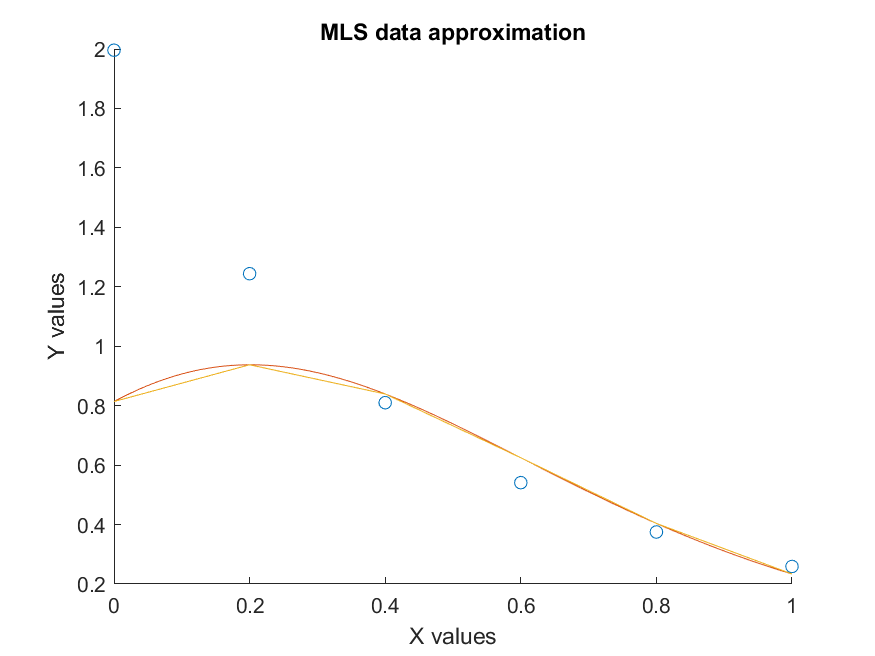
\includegraphics{./Problem5Fig.png}
\caption{}
\end{figure}

\section{Problem 6 MLS in Matlab}\label{problem-6-mls-in-matlab}

Given the dataset use the Matlab function polyfit to find respectively
the first, second, fourth, and eigth order polynomials using the method
of least squares. You should also plot your polynomials, together with
the data set.

Looking at the figure (fig 2), it is quite clear that increasing order
polynomials allow for lower error in the least squares sense.

Script

\begin{verbatim}
% Data Set
x = [0:0.1:1];
y = [0.7829 0.8052 0.5753 0.5201 0.3783 0.2923 0.1695 0.0842 0.0415 0.09 0];

% Polyfit 1, 2, 4, 8 order
first = polyfit(x,y,1);
second = polyfit(x,y,2);
fourth = polyfit(x,y,4);
eighth = polyfit(x,y,8);

% calculate model y values
yOne = polyval(first,x);
yTwo = polyval(second,x);
yFour = polyval(fourth,x);
yEight = polyval(eighth,x);

% plot on figure
figure
hold on
grid on
scatter(x,y)
plot(x,yOne);
plot(x,yTwo);
plot(x,yFour);
plot(x,yEight);
xlabel("X values");
ylabel("Y values");
title("MLS fitting at various orders");
legend('Data','First Order','Second Order','Fourth Order','Eight Order');
\end{verbatim}

Figure:

\begin{figure}
\centering
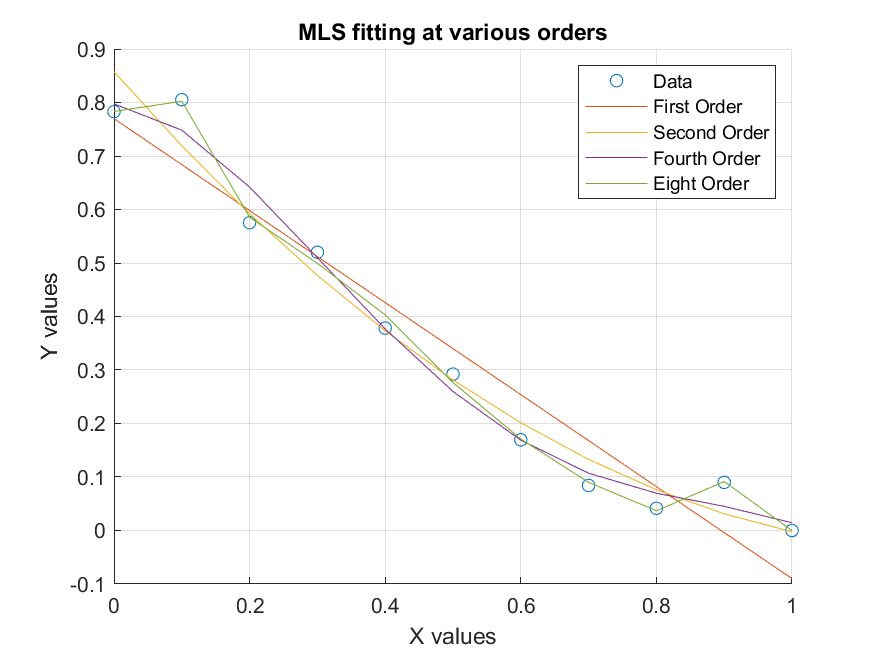
\includegraphics{./Problem6Figure.png}
\caption{}
\end{figure}

\section{Problem 7 Least squares approximation of
functions}\label{problem-7-least-squares-approximation-of-functions}

Let f(x) be a function defined on the interval {[}-1,1{]}, as

\[
f(x) = \begin{cases} 
    -1 & -1 \leq x < 0 \\
    1 & 0 \leq x\leq 1 
\end{cases}
\]

We want to approximate f(x) by a function of the form
\(g(x) = acos(\pi x) + bsin(\pi x)\). Find the best possible constants a
and b, by the method of least squares.

We know that the error function is:

\[
\int_{-1}^{1} (f(x)-g(x))^2dx
\] \[
\int_{-1}^{1} (f(x)-(acos(\pi x)+bsin(\pi x)))^2dx
\]

In order to minimize this error we must set the partial derivative with
respect to both a and b to zero.

\[
-2\int_{-1}^{1} cos(\pi x)(f(x)-(acos(\pi x)+bsin(\pi x)))dx
\] \[
-2\int_{-1}^{1} sin(\pi x)(f(x)-(acos(\pi x)+bsin(\pi x)))dx
\]

\[
-2\int_{-1}^{1} cos(\pi x)f(x)dx + 2\int_{-1}^{1}cos(\pi x)(acos(\pi x)+bsin(\pi x))dx
\] \[
-2\int_{-1}^{1} sin(\pi x)f(x)dx +2\int_{-1}^{1}sin(\pi x)(acos(\pi x)+bsin(\pi x))dx
\]

Since we want to set them equal to zero we can say:

\[
a\int_{-1}^{1}cos(\pi x)^2+b\int_{-1}^{1}cos(\pi x)sin(\pi x)dx=\int_{-1}^{1} cos(\pi x)f(x)dx
\] \[
a\int_{-1}^{1}sin(\pi x)cos(\pi x)+b\int_{-1}^{1}sin(\pi x)^2dx=\int_{-1}^{1} sin(\pi x)f(x)dx
\]

So now we make and solve our matrix. The values we need:

\[
\begin{array}{c|c|} 
\int_{-1}^{1}cos(\pi x)^2 & 1\\
\int_{-1}^{1}cos(\pi x)sin(\pi x)dx & 0\\
\int_{-1}^{1} cos(\pi x)f(x)dx & 0\\
\int_{-1}^{1}sin(\pi x)^2dx & 1\\
\int_{-1}^{1} sin(\pi x)f(x)dx & \frac4{\pi}\\
\end{array}
\]

This gives us the following matrix:

\[
\left(\begin{array}{cc} 
1 & 0\\
0 & 1
\end{array}\right)
\left(\begin{array}{c} 
a \\
b 
\end{array}\right) =
\left(\begin{array}{c}
0 \\
\frac4{\pi} 
\end{array}\right)
\]

This is already essentially solved, so the best possible constants a and
b for our function g(x) are \(a=0;b=\frac4{\pi}\). This gives us the
equation:

\[g(x) = \frac{4cos(\pi x)}{\pi}\]

Below is a graph of what the plot looks like (fig 3):

\begin{figure}
\centering
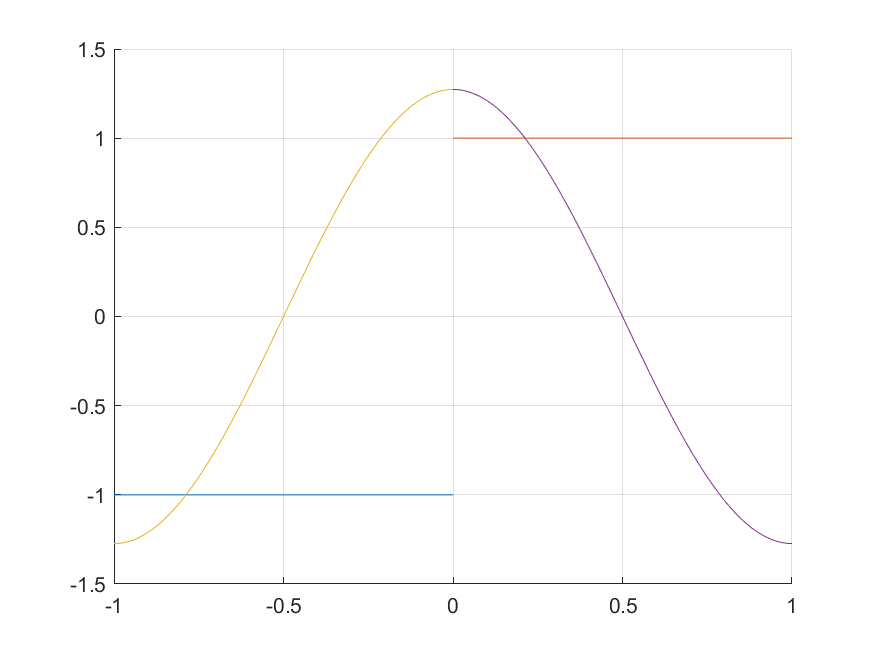
\includegraphics{./Problem7Figure.png}
\caption{}
\end{figure}


\end{document}
